\subsubsection{Dimensionierung}
Die Dimensionierung des Widerstandes $R_2$ in der Gegenkopplung erfolgte, bei
einer Verstärkung von $V = 11$ und einem Widerstand $R_1 = 10 \, \si{\kilo\ohm}$, durch
\[R_2 = \frac{R_1}{V - 1} = \frac{10 \, \si{\kilo\ohm}}{11 - 1} = 1 \, \si{\kilo\ohm}\]

\subsubsection{Übertragungskennlinie}
Die Übertragungskennlinie wurde durch Messung von Eingangs- und
Ausgangs(gleich)spannungen in einem Bereich von $-1.5 \, \si{\volt} \textrm{ bis
} 1.5 \, \si{\volt}$ bei einer Vergungsspannung von $\pm 15 \, \si{\volt}$ bestimmt und ist in Abb. \ref{fig:noninv} zu sehen.

\begin{figure}[H]
  \begin{center}
    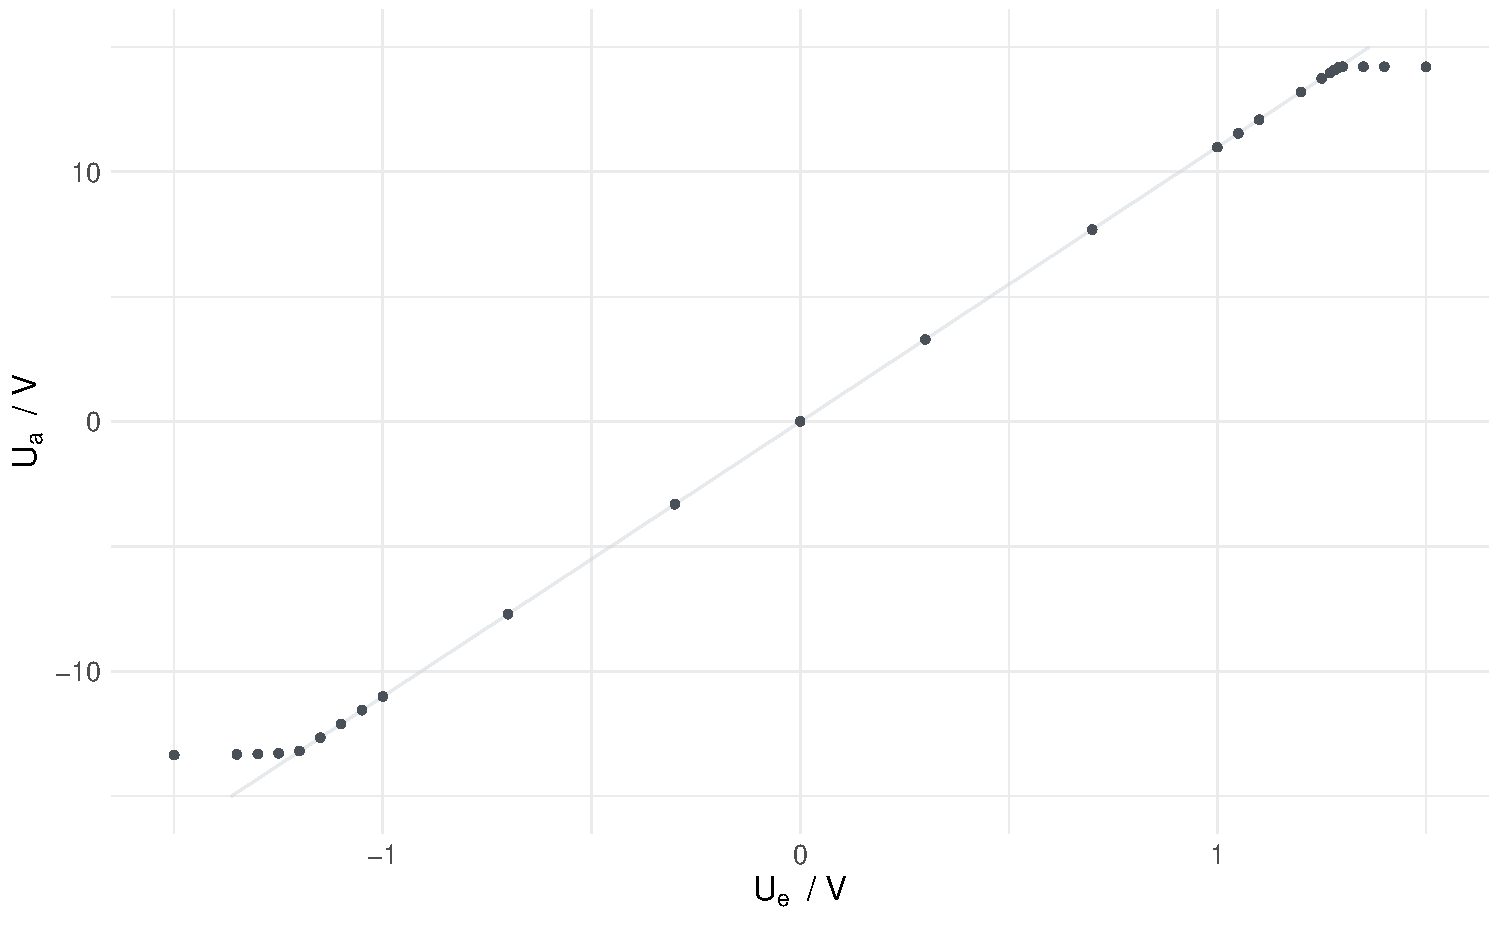
\includegraphics[width=\textwidth]{VERA/5_1/nichtinv.pdf}
  \end{center}
  \caption{Messtechnisch ermittelte Übertragungskennlinie}
  \label{fig:noninv}
\end{figure}

Die nichtinvertierende Charakteristik (positiver Eingang $\rightarrow$ positiver
Ausgang) ist zu erkennen. Der Anstieg der Geraden und damit die Verstärkung des
linearen Bereichs (vor der Sättigung) wurde durch eine Regressionsgerade
ermittelt und ist inetwa
\[V = 10.996\]

was sehr nahe an den theoretischen Verstärkungswert von $11$ herankommt.

Die Sättigung des Verstärkers beginnt in negative Richtung bei $U_e \approx
-1.25 \, \si{\volt}$ zu $U_a \approx 13.33 \, \si{\volt}$ und in positive
Richtung bei $U_e \approx 1.3 \, \si{\volt}$ zu $U_a \approx 14.2 \, \si{\volt}$.
Die Unsymmetrie könnte an einer unsymmetrischen Versorgungsspannung liegen,
leider wurde diese nicht nachgemessen, weshalb keine genaueren Aussagen getroffen
werden können.

\vspace{0.03444\paperheight}

% Please add the following required packages to your document preamble:
% \usepackage{booktabs}
\begin{table}[H]
  \begin{center}
\begin{tabular}{@{}ll@{}}
\toprule
$U_e / \si{\volt}$ & $U_a / \si{\volt}$ \\ \midrule
-1.5               & -13.349            \\
-1.35              & -13.32             \\
-1.3               & -13.303            \\
-1.25              & -13.277            \\
-1.2               & -13.184            \\
-1.15              & -12.653            \\
-1.1               & -12.103            \\
-1.05              & -11.554            \\
-1                 & -11.004            \\
-0.7               & -7.708             \\
-0.3               & -3.31              \\
0                  & 0.00999            \\ 
0.3                & 3.288              \\
0.7                & 7.688              \\
\end{tabular}
\hspace{0.1459\textwidth}
\begin{tabular}{@{}ll@{}}
1                  & 10.987             \\
1.05               & 11.537             \\
1.1                & 12.087             \\
1.2                & 13.187             \\
1.25               & 13.737             \\
1.27               & 13.96              \\
1.28               & 14.066             \\
1.29               & 14.174             \\
1.3                & 14.204             \\
1.35               & 14.205             \\
1.4                & 14.205             \\
1.5                & 14.205             \\ \bottomrule
  \end{tabular}
\end{center}
\caption{Messwerte der invertierenden Verstärkerschaltung}
\end{table}